Arimaa is played on a board composed of 64 tiles, like a chess board. As in chess, there are 6 types of pieces, but they are not those chess players are used to. From weakest to strongest, they are : rabbits (8 per player), cats, dogs, horses (2 of each per player), camels and elephants (one of each per player).

\begin{figure}[!h]
\centering

\includegraphics[width=\textwidth]{1_Presentation/1.1_Arimaa_rules_Gabriel/Pictures/Pieces.png}
\caption{The different piece types in Arimaa.}
\label{fig:pieces}
\end{figure}

Each player, starting with the gold player, places all of his pieces on the two back rows of his side. Then, the gold player takes the first turn.
On his turn, each player disposes of four moves. He or she can use these moves on a single piece, or on how many pieces as they desire.

All pieces can move on an adjacent square (but not diagonally), except for the rabbit which cannot move backwards.
A piece can instead use two moves to push or pull a weaker adjacent enemy piece, as shown in figure \ref{fig:displace}.

\begin{figure}[!h]
\centering
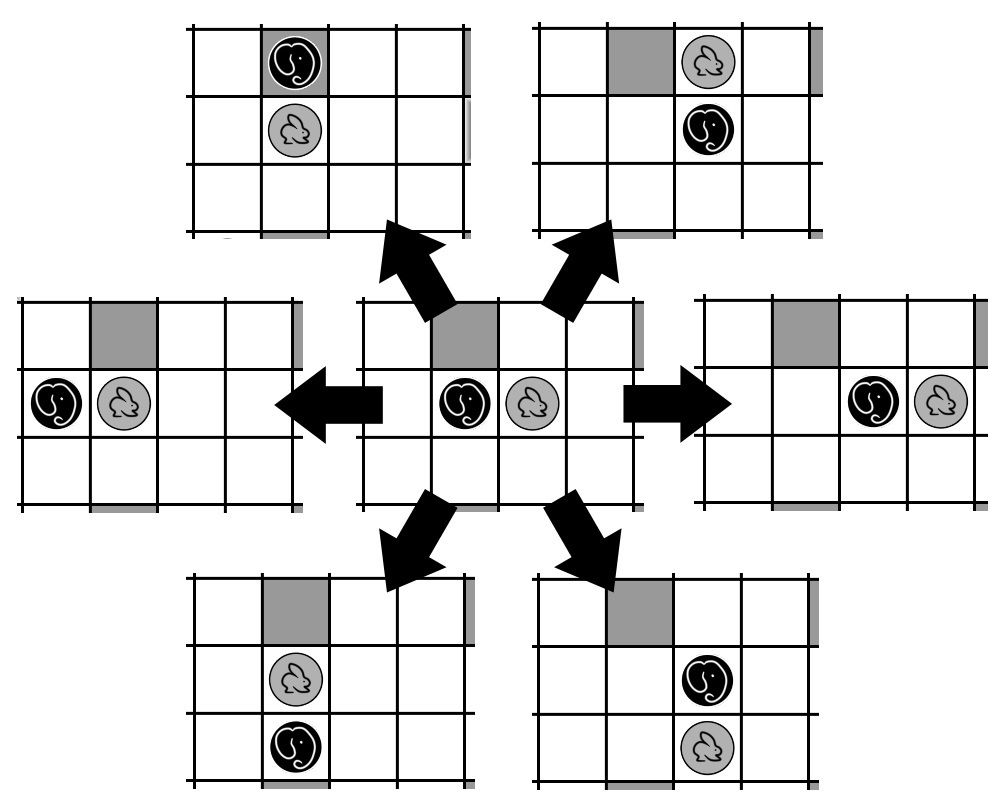
\includegraphics[width=0.6\textwidth]{1_Presentation/1.1_Arimaa_rules_Gabriel/Pictures/Displace.png}
\caption{The different ways you can push or pull a weaker enemy piece.}
\label{fig:displace}
\end{figure}

A piece sitting next to a stronger enemy piece is frozen. When a piece is frozen, it cannot move. As shown in figure \ref{fig:freeze}, a piece cannot be frozen while there is an ally piece beside it.

\begin{figure}[!h]
\centering
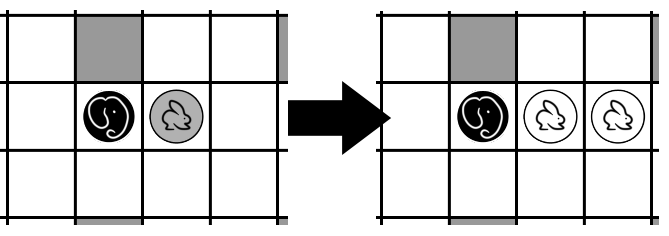
\includegraphics[width=0.5\textwidth]{1_Presentation/1.1_Arimaa_rules_Gabriel/Pictures/Freeze.png}
\caption[Example of the freezing mechanic.]{Example of the freezing mechanic. When the two rabbits are together, the one next to the elephant is no longer frozen.}
\label{fig:freeze}
\end{figure}

There are four traps on the board. As shown in figure \ref{fig:trap}, any piece sitting on a trap with no ally piece next to it dies.

\begin{figure}[!h]
\centering
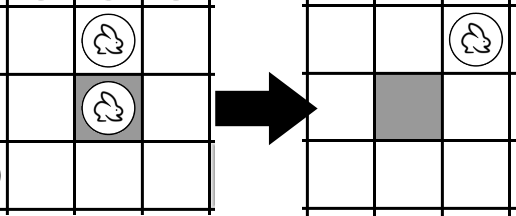
\includegraphics[width=0.5\textwidth]{1_Presentation/1.1_Arimaa_rules_Gabriel/Pictures/Trap.png}
\caption[Example of the traps mechanic.]{Example of the traps mechanic. As soon as there is no other ally pieces adjacent to the rabbit standing on the trap, it dies.}
\label{fig:trap}
\end{figure}

There are four ways to win the game:

\begin{description}
\item[Victory by reaching the goal:] A player wins the game if one of his rabbits reaches the other end of the board.
\item[Victory by elimination:] A player wins the game if he eliminates all the rabbits belonging to his opponent.
\item[Victory by elimination:] A player wins the game if his opponent can't make a move on his turn.
\item[Victory by repetition:] If the same position happens three times in a row, the player that makes it happen the third time loses the game.
\end{description}
